\documentclass{article}
\usepackage[utf8]{inputenc}
\usepackage{amsmath,amsthm,amssymb}
\usepackage{amsfonts}
\usepackage{arydshln}
\usepackage{enumitem}
\usepackage{float}
\usepackage{graphicx}
\usepackage{hyperref}
\usepackage{listings}
\usepackage{makecell}
\usepackage[margin=0.75in]{geometry}
\usepackage{mathtools} 
\usepackage{multicol}
\usepackage{subcaption}
\usepackage{wrapfig}
\allowdisplaybreaks
\newtheorem{theorem}{Theorem}
\newtheorem{lemma}{Lemma}

\DeclarePairedDelimiter{\abs}{\lvert}{\rvert}
\DeclarePairedDelimiter{\norm}{\lVert}{\rVert}

\usepackage{fancyhdr}
\pagestyle{fancy}
\fancyhf{}
\fancyhead[L]{Bridgette Delight}
\fancyhead[C]{Math 465 - Homework 04}
\fancyhead[R]{\thepage}
\renewcommand{\headrulewidth}{2pt}

\title{{\large Math 465}\\ Homework 0X}
\author{Bridgette Delight}
\date{\today}

\begin{document}

%\maketitle

\section{}
Suppose that the vector function $g=(g_1, \dots, g_n)$ is a contraction in the $p$-norm with $0<L<n^{-\frac{1}{p}}$ and $1 \le p \le \infty$. Show that $g$ is a contraction in the $\infty$-norm.

\begin{align*}
    \norm{x}_{p} &= \left( \sum_{i=1}^n |x_i|^p \right)^{\frac{1}{p}} \le \left( \sum_{i=1}^n\norm{x}_{\infty}^p \right)^{\frac{1}{p}} \\
    &= \left(\norm{x}_{\infty}^p \sum_{i=1}^n  1 \right)^{\frac{1}{p}}= \left( \norm{x}_{\infty}^p  \right)^{\frac{1}{p}}\\
    %%%%%%%%%%%%%%%%% here
    \norm{x}_{\infty} &\le  \left( \sum_{i=1}^{\infty} | x_i |^p \right)^{\frac{1}{p}} \\
    \norm{x}_{\infty}& \le  \norm{x}_{p} \le n^{\frac{1}{p}} \norm{x}_{\infty}\\
    \norm{g(x)- g(y)} & \le L \norm{x-y}_p \\
    \text{This is a contradiction}&\\
    \norm{g(x)- g(y)}_{\infty} & \le \norm{g(x)-g(y)}_p \le L \norm{x-y}_p \\
    &\le n^{\frac{1}{p}} L \norm{x-y}_{\infty} = w\cdot L \norm{x}_{\infty}\\
    w &= n^{\frac{1}{p}} \cdot L \\
    %%%%%%%%%%%%%%%%%% here
    &0 < L < n^{-\frac{1}{p}}<n^{\frac{1}{p}}\\
    &n^{\frac{1}{p}} \cdot L < 1\\
    0 &< n^{\frac{1}{p}\cdot L}<1\\
    \norm{g(x) - g(y)}_{\infty} & \le n^{\frac{1}{p}} \cdot L \norm{x - y}_{\infty}\\
    &= w \norm{ x - y }_{\infty} \\
    \text{So, $\norm{g}_{\infty}$ is a contraction}&\\
\end{align*}


\section{}
Suppose $f: \mathbb{R}^n \to \mathbb{R}^n$ and that $\xi \in \mathbb{R}^n$ is such that $f(\xi )=0$. Suppose $f$ is continuous in a certain neighborhood of $\xi$ and that the Jacobian matrix $J_f(x)$ is invertible at $x=\xi$ (so it is invertible at $x$ close to $\xi$). Let $\textbf{K}(x)=[J_f(x)]^{-1}$, and define the sequence $\bigg\{x^k \bigg\}_{k=0}^{\infty} \subset \mathbb{R}^n$ by
\begin{equation*}
    \begin{cases}
    x^0 \text{ is such that }\textbf{K}(x_0) \text{ exists}\\
    x^{k+1}=g(x^k), & k=0,1,2,\dots ,
    \end{cases}
\end{equation*}
where $g(x) = x-\textbf{K}(x)f(x)$.
\begin{enumerate}[label = (\alph*)]
    \item Show that the Jacobian matrix $J_g(x)=[\gamma_{ij}]_{i,j=0}^n$ of $g$ is given by the formula
    \begin{equation*}
        \gamma_{ij} = \delta_{ij} - \sum_{r=1}^n \frac{\partial \textbf{K}_{ir}}{\partial x_j}f_r - \sum_{r=1}^n \textbf{K}_{ir}J_{rj},
    \end{equation*}
    with $[J_{rj}]_{r,j=0}^n = J_f(x)$, $\delta_{ij} = 0$ if $i \ne j$ and $\delta_{ij}=1$ if $i=j$.
    \item Use the result of part (a) to show that all elements of $J_g(\xi)$ are identically zero.
\end{enumerate}

\subsection*{(2a)}

\begin{align*}
    g(x) &= x- K(x)f(x)\\
    g(x) &= 
    \begin{bmatrix} 
    k_{11}(x) & k_{12}(x) &  k_{13}(x) & \dots &  k_{1n}(x) \\[1ex]
    k_{21}(x) & k_{22}(x) &  k_{23}(x) & \dots &  k_{2n}(x) \\[1ex]
    k_{31}(x) & k_{32}(x) &  k_{33}(x) & \dots &  k_{3n}(x) \\[1ex]
    \vdots & \vdots & \vdots & \dots & \vdots \\[1ex]
    k_{n1}(x) & k_{n2}(x) &  k_{n3}(x) & \dots &  k_{nn}(x) \\[1ex]
    \end{bmatrix}
    \begin{bmatrix}
    f_1(x)\\[1ex]
    f_2(x)\\[1ex]
    f_3(x)\\[1ex]
    \vdots \\[1ex]
    f_n(x)\\[1ex]
    \end{bmatrix}\\
    %%%% end matrix
    g_i(x) &= x_i - \bigg( k_{i1}(x)f_1(x)+k_{i2}(x)f_2(x) + k_{i3}(x)f_3(x) + \dots + k_{in}(x)f_n(x)\bigg)\\
    \frac{\partial g_i}{\partial x_j} &= \frac{\partial x_i}{\partial x_j} - \frac{\partial}{\partial x_j}\bigg( k_{i1}(x)f_1(x)+k_{i2}(x)f_2(x) + k_{i3}(x)f_3(x) + \dots + k_{in}(x)f_n(x)\bigg)\\
    &= \frac{\partial x_i}{\partial x_j} - \sum_{r=1}^n \frac{\partial x_{ir}}{\partial x_j}(x) f_r (x) - \sum_{r=1}^n k_{ir}^n J_{rj}(x)\\ 
    [J_{rj}]_{r,j=1}^n &= J_f(x) \\
    \text{when $i=j$}&\\
    & \frac{\partial x_i}{\partial x_j} =  \frac{\partial x_i}{\partial x_i} = 1 \\
     \text{when $i\ne j$}&\\
     &\frac{\partial x_i}{\partial x_j}  = 0 \\
     \text{So,}&\\
     J_g(x) &= [\gamma_{ij}]_{i,j=1}^n\\
     \gamma_{ij} &= \delta_{ij} - \sum_{r=1}^n \frac{\partial K_{ir}}{\partial x_j}f_r - \sum_{r=1}^n k_{ir}J_{rj}\\
     \text{when }\delta_{ij}&= 1 \quad \text{when }i=j \quad \text{and }\delta_{ij}= 1  \text{when } i \ne j \\
\end{align*}

\subsection*{(2b)}

\begin{align*}
    f(\xi) &= \Vec{0}\\
    \delta_{ij} & = 
    \begin{bmatrix}
    1 & 0 &0 & \dots &0 \\[1ex]
    0 & 1 &0 & \dots &0 \\[1ex]
    \vdots & \vdots &\vdots &\vdots & 0 \\[1ex]
    0 & 0 &0 &0 & 1 \\[1ex]
    \end{bmatrix} = I \\
    \Vec{0} &= \sum_{r=1}^n \frac{\partial k_{ir}(\xi)}{\partial x_j} f_r(\xi) \\
    k_{ir}(\xi) &= J_{ij}^{-1}(\xi)\\
    I &= \sum_{r=1}^n J_{ij}^{-1}(\xi) \cdot J_{rj}(\xi) \\
    \text{Thus,}&\\
    \Vec{0} &= I - \Vec{0} - I \\
    J_g (\xi) &= \Vec{0}\\
\end{align*}

\section{}
Let $f:\mathbb{R}^2 \to \mathbb{R}^2$ be defined by $f(x_1,x_2)= (x_1^2 + x_2^2-2, \quad x_1 - x_2)$.
\begin{enumerate}[label = (\alph*)]
    \item Solve the system $f(x_1.x_2)=0$.
    \item Consider the iterative process
    \begin{equation}
        \label{q3b}
        x^{k+1} = x^l - [J_f(x)]^{-1}f(x^k), \quad k=0,1,2,\dots
    \end{equation}
    where $J_f$ is the Jacobian of $f$, and show that for $k=0$,
    \begin{equation*}
        x_1^1 = x_2^1 = \frac{(x_1^0)^2+(x_2^0)^2+2}{2(x_1^0+x_2^0)}.
    \end{equation*}
    \item Show that
    \begin{equation*}
        \text{if } x_1^0 + x_2^0 >0 \text{ then } 
        \begin{pmatrix} x_1^k \\[1ex] x_2^k\\[1ex] \end{pmatrix} \to \begin{pmatrix} 1 \\[1ex] 1\\[1ex] \end{pmatrix} \text{ as } k \to \infty
    \end{equation*}
    and
    \begin{equation*}
        \text{if } x_1^0 + x_2^0 <0 \text{ then } 
        \begin{pmatrix} x_1^k \\[1ex] x_2^k\\[1ex] \end{pmatrix} \to \begin{pmatrix} -1 \\[1ex] -1\\[1ex] \end{pmatrix} \text{ as } k \to \infty
    \end{equation*}
    \item Run the algorithm (\ref{q3b}) with $x_1^0 = 2$, $x_2^0=3$ and present a figure showing $x_1^k$ and $x_2^k$ (vertical axis) versus $k=0,1,2,\dots ,10$ (horizontal axis).
\end{enumerate}


\subsection*{(3a)}

\begin{align*}
    x_1 - x_2 = 0 \quad &\text{and, }x_1^2 + x_2^2 - 2 =0\\
    \text{So,}&\\
    x_1 &= x_2 \\
    \text{Substitute $x_1 = x_2 $}&\\
    0 &= x_2^2 + x_2^2 - 2\\
    2 &= x_2^2 + x_2^2\\
    2 &= 2x_2^2\\
    x_2 &= \pm 1\\
    \begin{bmatrix} x_1 \\ x_2 \end{bmatrix} &= \begin{bmatrix} 1 \\ 1 \end{bmatrix} \text{ or } \begin{bmatrix} -1 \\ -1 \end{bmatrix}\\
\end{align*}

\subsection*{(3b)}

\begin{align*}
    \begin{bmatrix} x_1^1 \\[1ex] x_2^1\end{bmatrix} &= \begin{bmatrix} x_1^0 \\[1ex] x_2^0\end{bmatrix} - \begin{bmatrix} 2x_1^0 & 2x_2^0 \\[1ex] 1 & -1\end{bmatrix} \cdot \begin{bmatrix} (x_1^0)^2+(x_2^0)^2 -2 \\[1ex] x_1^0 - x_2^0 \end{bmatrix} \\
    \begin{bmatrix} x_1^1 \\[1ex] x_2^1\end{bmatrix} &=  \begin{bmatrix} x_1^0- \frac{(x_1^0)^2 + (x_2^0)^2 -2}{2(x_1^0+x_2^0)} - \frac{x_2^0 (x_1^0 - x_2^0)}{x_1^0 + x_2^0} \\[1ex] x_2^0 - \frac{(x_1^0)^2 + (x_2^0)^2 -2}{2(x_1^0+x_2^0)} - \frac{x_1^0 (x_1^0 - x_2^0)}{x_1^0 + x_2^0} \end{bmatrix} \cdot  \\
    x_1^1 &=  \frac{x_1^0(2(x_1^0 + x_2^0))}{2(x_1^0+x_2^0)} - \frac{(x_1^0)^2 + (x_2^0)^2 - 2 }{2(x_1^0+x_2^0)} - \frac{2x_2^0(x_1^0 - x_2^0)}{2(x_1^0+x_2^0)} \\
    &= \frac{x_1^0(2(x_1^0 + x_2^0))-(x_1^0)^2 - (x_2^0)^2 + 2 - x_2^0(x_1^0 - x_2^0)}{2(x_1^0+x_2^0)}\\
    &=  \frac{2(x_1^0)^2 + 2x_1^0x_2^0 - (x_1^0)^2 - (x_2^0)^2 +2 - 2x_1^0x_2^0 + 2(x_2^0)^2}{2(x_1^0+x_2^0)}\\
    &=  \frac{(x_1^0)^2 + (x_2^0)^2 + 2 }{2(x_1^0+x_2^0)}\\
    x_2^1 &=  \frac{x_2^0(2(x_1^0 + x_2^0))}{2(x_1^0+x_2^0)} - \frac{(x_1^0)^2 + (x_2^0)^2 - 2 }{2(x_1^0+x_2^0)} + \frac{2x_1^0(x_1^0 - x_2^0)}{2(x_1^0+x_2^0)} \\
    &= \frac{x_2^0(2(x_1^0 + x_2^0))-(x_1^0)^2 - (x_2^0)^2 + 2 + x_1^0(x_1^0 - x_2^0)}{2(x_1^0+x_2^0)}\\
    &= \frac{2x_1^0x_2^0 + 2(x_2^0)^2 - (x_1^0)^2 - (x_2^0)^2 + 2 + 2(x_1^0)^2 - 2x_1^0x_2^0}{2(x_1^0+x_2^0)}\\
    &= \frac{(x_1^0)^2 + (x_2^0)^2 +2}{2(x_1^0 + x_2^0)}\\
    \text{Thus,}&\\
    x_1^1 &= x_2^2 =  \frac{(x_1^0)^2 + (x_2^0)^2 +2}{2(x_1^0 + x_2^0)}\\
\end{align*}

\subsection*{(3c)}

\begin{align*}
    0 &< x_1^0 + x_2^0 \\
    x_1^1 &= x_2^1 > 0 \\
    x_1^k &= x_2^k >0\\
    x^{k+1} &> x^k \\
    x^{k+1} &= \frac{(x_1^k)^2 + (x_2^k)^2 + 2}{2(x_1^k + x_2^k)}\\
    x_1^k & \le \frac{(x_1^k)^2 + (x_2^k)^2 + 2}{2(x_1^k + x_2^k)}\\
    x^k & \le \frac{(x_1^k)^2 + (x_2^k)^2 + 2}{2(x_1^k + x_2^k)}\\
    \text{We will say $x_1^k = x_2^k = x^k$ for easier reading}&\\
    x^k & \le \frac{(x^k)^2 +1}{2x^k}\\
    2(x^k)^2 & \le (x^k)^2 +1  \\
    2(x^k)^2 & \le 1 \\
    \text{So, $0 <x^k \le 1$ is monotonically increasing.}&\\
    0 & > x_1^0 + x_2^0 \\
    x_1^0 &= x_2^0 < 0 \\
    x_1^k &= x_2^k \\
    x_1^k & \ge \frac{(x_1^k)^2 + (x_2^k)^2 + 2}{2(x_1^k + x_2^k)}\\
    \text{We will say $x_1^k = x_2^k = x^k$ for easier reading}&\\
    x^k & \ge  \frac{(x^k)^2 +1}{2x^k}\\
    (x^k)^2 & \le 1 \\
    \text{So, $-1 \le x^k < 0$ is monotonically decreasing.}&\\
    \text{Since,}&\\
    x^{k+1} & \ge x^k\\
    \lim_{k \to \infty} x^k &= \lim_{k \to \infty} 1\\
    &= 1\\
     \text{Since,}&\\
    x^{k+1} & \le x^k\\
    \lim_{k \to \infty} x^k &= \lim_{k \to \infty} -1\\
    &= -1\\
    \text{Thus, it is bounded.}
\end{align*}

\subsection*{(3d)}

\begin{figure}[H]
    \centering
    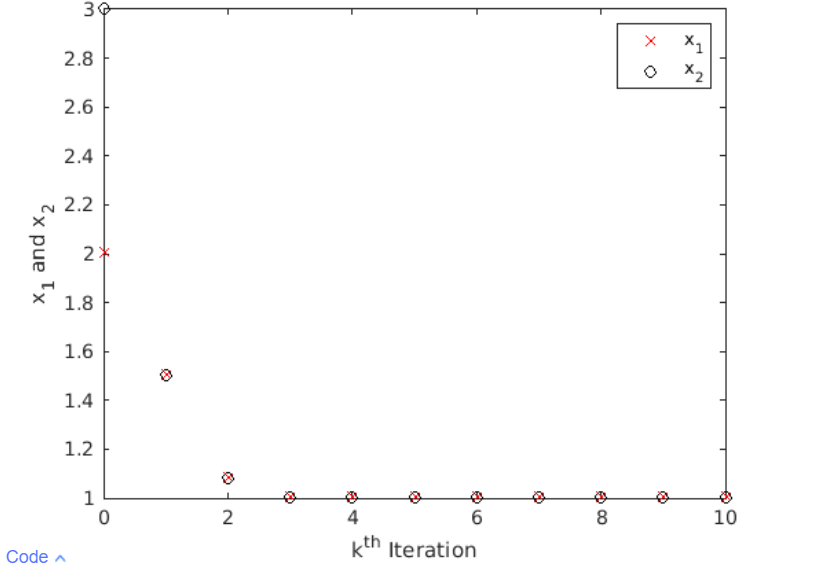
\includegraphics[width = .75\linewidth]{images/hw04q3d.PNG}
    \caption{$k^{th}$ iteration}
    \label{fig:my_label}
\end{figure}


\end{document}